\documentclass[11pt,a4paper]{article}

% === Encoding & Font ===
\usepackage[T1]{fontenc}
\usepackage[utf8]{inputenc}
\usepackage{mathpazo}                                    % Palatino (NBER style)
\usepackage[protrusion=true,expansion=true]{microtype}   % optical margins

% === Layout ===
\usepackage[top=2cm, bottom=1.5cm, left=1.8cm, right=1.8cm]{geometry}
\usepackage{setspace}
\setstretch{1.05}

% === Widow/orphan control ===
\widowpenalty=10000
\clubpenalty=10000

% === Math ===
\usepackage{amsmath,amssymb}

% === Figures ===
\usepackage{graphicx}
\usepackage{float}
\usepackage{xcolor}
\usepackage[font=small, labelfont=bf, labelsep=period]{caption}
\usepackage{mdframed}

% === Tables ===
\usepackage{booktabs}
\usepackage{tabularx}
\usepackage{colortbl}

% === Multi-column (biblio) ===
\usepackage{multicol}

% === Section spacing ===
\usepackage{titlesec}
\titlespacing*{\section}{0pt}{10pt plus 2pt minus 2pt}{4pt plus 2pt minus 1pt}

% === Figure spacing ===
\setlength{\intextsep}{4pt plus 1pt minus 1pt}
\setlength{\abovecaptionskip}{6pt}
\setlength{\belowcaptionskip}{3pt}

% === Transition blocks ===
\newcommand{\bridgeskip}{\vspace{6pt}}

% === Bibliography ===
\usepackage[numbers,sort&compress]{natbib}
\bibliographystyle{ieeetr}

% === URLs in references ===
\usepackage{url}

% === Hyperlinks (load last) ===
\usepackage[colorlinks=false]{hyperref}

% === Header/footer (NBER working paper style) ===
\usepackage{fancyhdr}
\pagestyle{fancy}
\fancyhf{}
\fancyhead[L]{\small\itshape Hatmi --- The Flattening}
\fancyhead[R]{\small\itshape Risk Prize 2026}
\fancyfoot[C]{\small\thepage}
\renewcommand{\headrulewidth}{0.4pt}

% First page: no header, just page number
\fancypagestyle{plain}{%
  \fancyhf{}
  \fancyfoot[C]{\small\thepage}
  \renewcommand{\headrulewidth}{0pt}
}

% ============================================================
\begin{document}

% ============================================================
% PAGE DE GARDE (page 1 — pas de header running)
% ============================================================
\thispagestyle{plain}
\vspace*{\fill}

\begin{center}
\begin{tabular*}{\textwidth}{@{}c@{\extracolsep{\fill}}c@{\extracolsep{\fill}}c@{}}
$\vcenter{\hbox{
\includegraphics[height=1.3cm]{../logo/ucam-logo-colour-preferred.png}}}$ &
$\vcenter{\hbox{
\includegraphics[height=1.4cm]{"../logo/CentraleSup Logo H_RVB.png"}}}$ &
$\vcenter{\hbox{
\includegraphics[height=1.3cm]{../logo/01_Horizontal.png}}}$
\end{tabular*}
\end{center}

\vspace{0.4cm}

\begin{center}
{\LARGE\bfseries The Flattening: When AI Productivity Gains\\[4pt]Conceal Tail Risk}\\[10pt]
{\large Bilel Hatmi}\\[4pt]
{\normalsize Part III Mathematical Statistics\\[2pt]
University of Cambridge\\[2pt]
{\small CentraleSup\'{e}lec~--~Universit\'{e} Paris-Saclay}}\\[6pt]
{\normalsize March 2026}\\[5pt]
\textit{Submitted to the Cambridge--McKinsey Risk Prize 2026}
\end{center}

\vspace{0.5cm}
\noindent\rule{\textwidth}{0.5pt}
\vspace{0.3cm}

\begin{abstract}
Generative AI improves average decision quality in organisations. It also
amplifies their worst-case exposure, through a mechanism that current
productivity metrics cannot capture.
Two channels produce this outcome. Algorithmic screening homogenises cognitive
profiles at entry. Cognitive surrender erodes independent judgment from within.
Both raise the error correlation across decision-makers, which is what drives
tail losses.
A Monte Carlo stress test of 200 agents over 20 quarters quantifies the gap:
average errors fall by 38\% while worst-case quarterly losses rise by 56\%,
masked by a 54\% productivity gain. The model was validated by two independent
implementations converging within 2\%.
The most actionable single intervention is AI provider diversification, which
cuts the tail risk premium by approximately 15\%. It is a procurement decision,
implementable in weeks. Yet without regulation, the Nash equilibrium is
unmanaged adoption for all firms: individually rational, collectively
catastrophic. The diversity of independent judgment that makes organisational
governance possible is being depleted faster than any single firm has
incentive to preserve it.
\end{abstract}



\vspace{0.5cm}
\noindent\rule{\textwidth}{0.5pt}

\vspace*{\fill}
\clearpage

% ============================================================
\section{The paradox your dashboard hides}

Nine participants in a product-design experiment asked ChatGPT to help them invent
a toy.
All nine named it ``Build-a-Breeze Castle.''
Without AI, every participant produced a unique concept.
With AI, 94\% of ideas shared the same building blocks; only 6\% remained
distinct~\cite{meincke_nhb_2025}.
Each individual output improved.
The collective output collapsed.

This is not a quirk of one experiment.
The Diversity Prediction Theorem decomposes collective error into two terms:
average individual error, and the diversity of individual
errors~\cite{page_princeton_2007,krogh_nips_1995}.
When AI reduces the first term but collapses the second, collective error rises
mechanically.
The variance of aggregate losses follows:
\[
  \text{Var}(L) = NK\,\bar{p}(1-\bar{p})\bigl(1 + (NK-1)\bar{\rho}\bigr)
\]
\noindent Even a modest rise in $\bar{\rho}$, the mean pairwise error correlation
across employees, drives the tail~\cite{wood_jmlr_2023}.
A preprint meta-analysis of 379 experimental conditions quantifies the trade-off:
AI raises individual creative performance by $g = +0.27$ but collapses collective
diversity by $g = -0.86$~\cite{holzner_arxiv_2025}.
The loss of diversity is three times the gain in performance.
Carlson and Doyle call such systems robust-yet-fragile~\cite{carlson_prl_2000}:
optimised for the frequent case, exposed to the rare one.
In most quarters, errors stay scattered and small.
In crisis quarters, they correlate and aggregate.
The loss distribution splits into two regimes, and the mean falls in a gap between
them where almost no actual quarter lies.

The paradox has a second property that matters more for risk managers: it is
concealed by the same productivity metrics that appear to confirm performance.

This essay addresses the CRO who sees a 54\% productivity gain on the dashboard
but cannot yet see the 94\% rise in risk-adjusted worst-case losses behind it.
The argument applies to any AI system that standardises the inputs to
organisational decisions, from legacy algorithmic screening tools to generative
models deployed in knowledge work.
Under unmanaged adoption, average decision errors fall by 38\% while worst-case
quarterly losses rise by 56\%.
The productivity shock that improves the mean simultaneously expands the volume of
decisions exposed to correlated failure.
The risk-adjusted $P_{99}$ rises by 94\%.
The dashboard records the gain; the tail accumulates off-screen.
For elite firms, those whose employees outperform AI outside its competence
frontier, the masking is more extreme: a 192\% rise in risk-adjusted tail exposure
against 18\% apparent productivity growth.
The dashboard cannot distinguish speed from accuracy.

This exposure is not distributed randomly.
It is structurally determined, and for the roughly 100{,}000 mid-market
organisations in the US and the EU most at risk, it is approaching without
a governance framework to navigate it.

This essay does three things for decision-makers.
First, it identifies the two mechanisms that produce the trap.
Second, it maps exposure across organisational profiles, showing that the perceived
worst-case risk is nearly half the actual exposure, and that tail risk varies
structurally across firms in the same sector with the same talent.
Third, it distributes three governance levers across three distinct actors, one
of which is a procurement decision actionable in weeks.

\bridgeskip
\noindent\emph{Two channels produce this outcome. One operates at the point of entry. The other
operates from within. Both converge on the same structural target: the correlation
of errors across decision-makers.}

% ============================================================
\section{Two channels, one target}

Human hiring was a porous filter. Interviewers disagreed, biases cancelled
partially, and non-linear profiles slipped through. AI screening is not a better
version of this process. It is a different kind of process: systematic, coherent,
and closed.
Fuller et al.\ document 27 million Americans excluded from consideration by
automated tracking systems, including caregivers, veterans, and career-changers
screened out by rigid keyword matching~\cite{fuller_hbs_2021}.
The bias is not confined to one model or one protected category.
Five major LLMs evaluating 361{,}000 r\'{e}sum\'{e}s exhibit strikingly similar
bias patterns~\cite{an_pnasnexus_2025,glazko_facct_2024,wilson_aies_2024}: the
filter industrialises what each training corpus encodes.
These models learn from the same corpora that reflect decades of cultural matching
in elite professional hiring~\cite{rivera_asr_2012}.
Schneider's attraction-selection-attrition model~\cite{schneider_pp_1987} predicts
the outcome: organisations converge toward cognitive homogeneity.
AI accelerates the convergence.

This convergence does not merely narrow representation. It correlates errors.
Across major language models, 60\% of mistakes are already
shared~\cite{kim_icml_2025}. Even before human homogenisation, the tools themselves
fail together.
Add cognitively convergent workforces recruited through the same filter, and the
errors of persons and the errors of tools superimpose in the same direction at the
same moment.

The pattern is not new. In 1998, Long-Term Capital Management lost \$4.6 billion
in four months. The fund employed Nobel laureates and PhD physicists who had
converged on identical arbitrage
strategies~\cite{jorion_efm_2000,mackenzie_econsoc_2003}. The problem was not
a lack of intelligence. It was a lack of diversity. In 2008, banks used the
same risk models, the same Value-at-Risk parameters, the same copula assumptions.
Homogeneity bred fragility~\cite{haldane_nature_2011}. In July 2024, a single
CrowdStrike update crashed 8.5 million Windows machines in
78 minutes~\cite{microsoft_crowdstrike_2024}, costing Fortune~500 firms an
estimated \$5.4~billion~\cite{parametrix_crowdstrike_2024}.
Geer et al.~\cite{geer_ccia_2003} had predicted software monoculture risk
twenty-one years earlier.
The mechanism is the same across all three episodes: when diversity collapses,
losses stop compensating and start aggregating. Kleinberg and Raghavan formalise
the point: even when an algorithm is individually superior, convergence on the
same algorithm degrades collective welfare~\cite{kleinberg_pnas_2021}.

This is the entry channel. A second channel operates on those already inside.

The employees who pass the filter progressively surrender the independence they
retain. Shaw and Nave document the phenomenon in a preprint study of 1{,}372
participants across 9{,}593 trials~\cite{shaw_psyarxiv_2026}.
When the AI errs, 79.8\% of participants follow its recommendation anyway.
The asymmetry is stark: correct AI advice raises accuracy by 25.2 percentage
points, but incorrect AI advice reduces it by only 14.3 points, a Cohen's
$h$ of~0.81.
Confidence rises by 11.7 points even when AI accuracy is 50\%, and does not decay
with experience ($p = 0.202$).
What makes this dangerous is not the surrender itself but the fact that confidence
rises alongside it.
Dell'Acqua et al.\ replicate the pattern among 758 consultants in a field
experiment~\cite{dellacqua_orgscience_2026}: inside the AI's competence frontier,
quality improves by 40\%. Outside it, accuracy drops 19 percentage points. The
most AI-skilled consultants perform worst, because competence in using the tool
compounds the surrender.
Professionals are not immune. In a randomised trial, radiologists exposed to biased
AI recommendations degraded their diagnostic accuracy by 11.3 percentage
points~\cite{jabbour_jama_2023}.
Passive scaffolding changes nothing: 93\% of clinical decision-support alerts are
overridden without review~\cite{bryant_aci_2014}. Bainbridge identified this as
the central irony of automation four decades ago~\cite{bainbridge_automatica_1983}:
removing humans from the control loop degrades the competence required to reenter it.

Keck and Tang provide the experimental link between both
channels~\cite{keck_psychsci_2020}: groups combining diverse cognitive processes
exhibit near-zero inter-judge error correlations, while homogeneous groups produce
strongly correlated errors.
Screening eliminates the structural source of that decorrelation.
Surrender erodes the behavioural independence that remains.
The Diversity Prediction Theorem delivers the consequence: as the diversity term
vanishes, collective error rises even as individual error falls.
The property is symmetric. When AI is right, correlated followers cluster at the
same correct answer. When AI errs, they cluster at the same wrong
answer, simultaneously, at scale.
This is what produces the bimodal distribution introduced in Section~1: in normal
quarters, correlated successes hold losses low; in crisis quarters, correlated
errors drive them high. The mean falls in a gap between two regimes that rarely
overlap.
One caveat: this link assumes that cognitive-profile diversity proxies for
cognitive-process diversity in real organisations, an inference that is plausible
but untested.

\bridgeskip
\noindent\emph{The mechanism is identified, and both channels are empirically grounded.
What remains is the magnitude. A Monte Carlo stress test answers that question
next.}

% ============================================================
\section{Quantifying the hidden exposure}

We simulate an organisation of 200 employees, each characterised by a cognitive
type $\tau_i \sim \mathrm{Beta}(2,2)$ on $[0,1]$ and a skill level
$h_i(t) \sim U(0.4, 0.8)$.
Each quarter, the organisation faces ten decisions in a stochastic environment
where the fraction of tasks inside the AI's competence frontier follows a
two-regime mixture: a normal regime in 92\% of quarters and a crisis regime in
8\%, in which the frontier shift and the systemic error shock are coupled. This
is the conditional stress logic of Basel~II applied to cognitive errors rather
than credit defaults.
Inter-decision error correlation follows the Vasicek single-factor
structure~\cite{vasicek_risk_2002}, the standard Basel~II/III framework for
modelling correlated failures.

Four governance scenarios are compared.
G0 adopts AI without governance: employees consult freely, no independent judgment
required.
G1 introduces passive scaffolding: alert flags signal low-confidence outputs, with
no compliance requirement.
G2 implements active scaffolding: employees record an independent judgment before
consulting the AI.
The model runs several hundred independent replications, validated by two
implementations converging within 2\%.
It is a stress test, not a forecast. It demonstrates that the mechanism \emph{can}
produce the paradox under plausible parameters, not that it does so in every
organisation.

Consider what a manager actually observes.
Quarterly performance follows the left mode in 92\% of quarters.
The manager's empirical estimate of tail risk, the worst quarter they have ever
seen, is built from these observations alone.
The perceived $P_{99}$, calculated on normal-regime quarters only, stands near
877.9.
The actual $P_{99}$ under unmanaged adoption is 1{,}714: a factor of nearly two
($\times$1.95). Figure~\ref{fig:bimodal} shows the full distribution.

\begin{figure}[H]
\begin{mdframed}[linewidth=0.5pt, linecolor=black!30, innertopmargin=6pt, innerbottommargin=2pt]
  \centering
  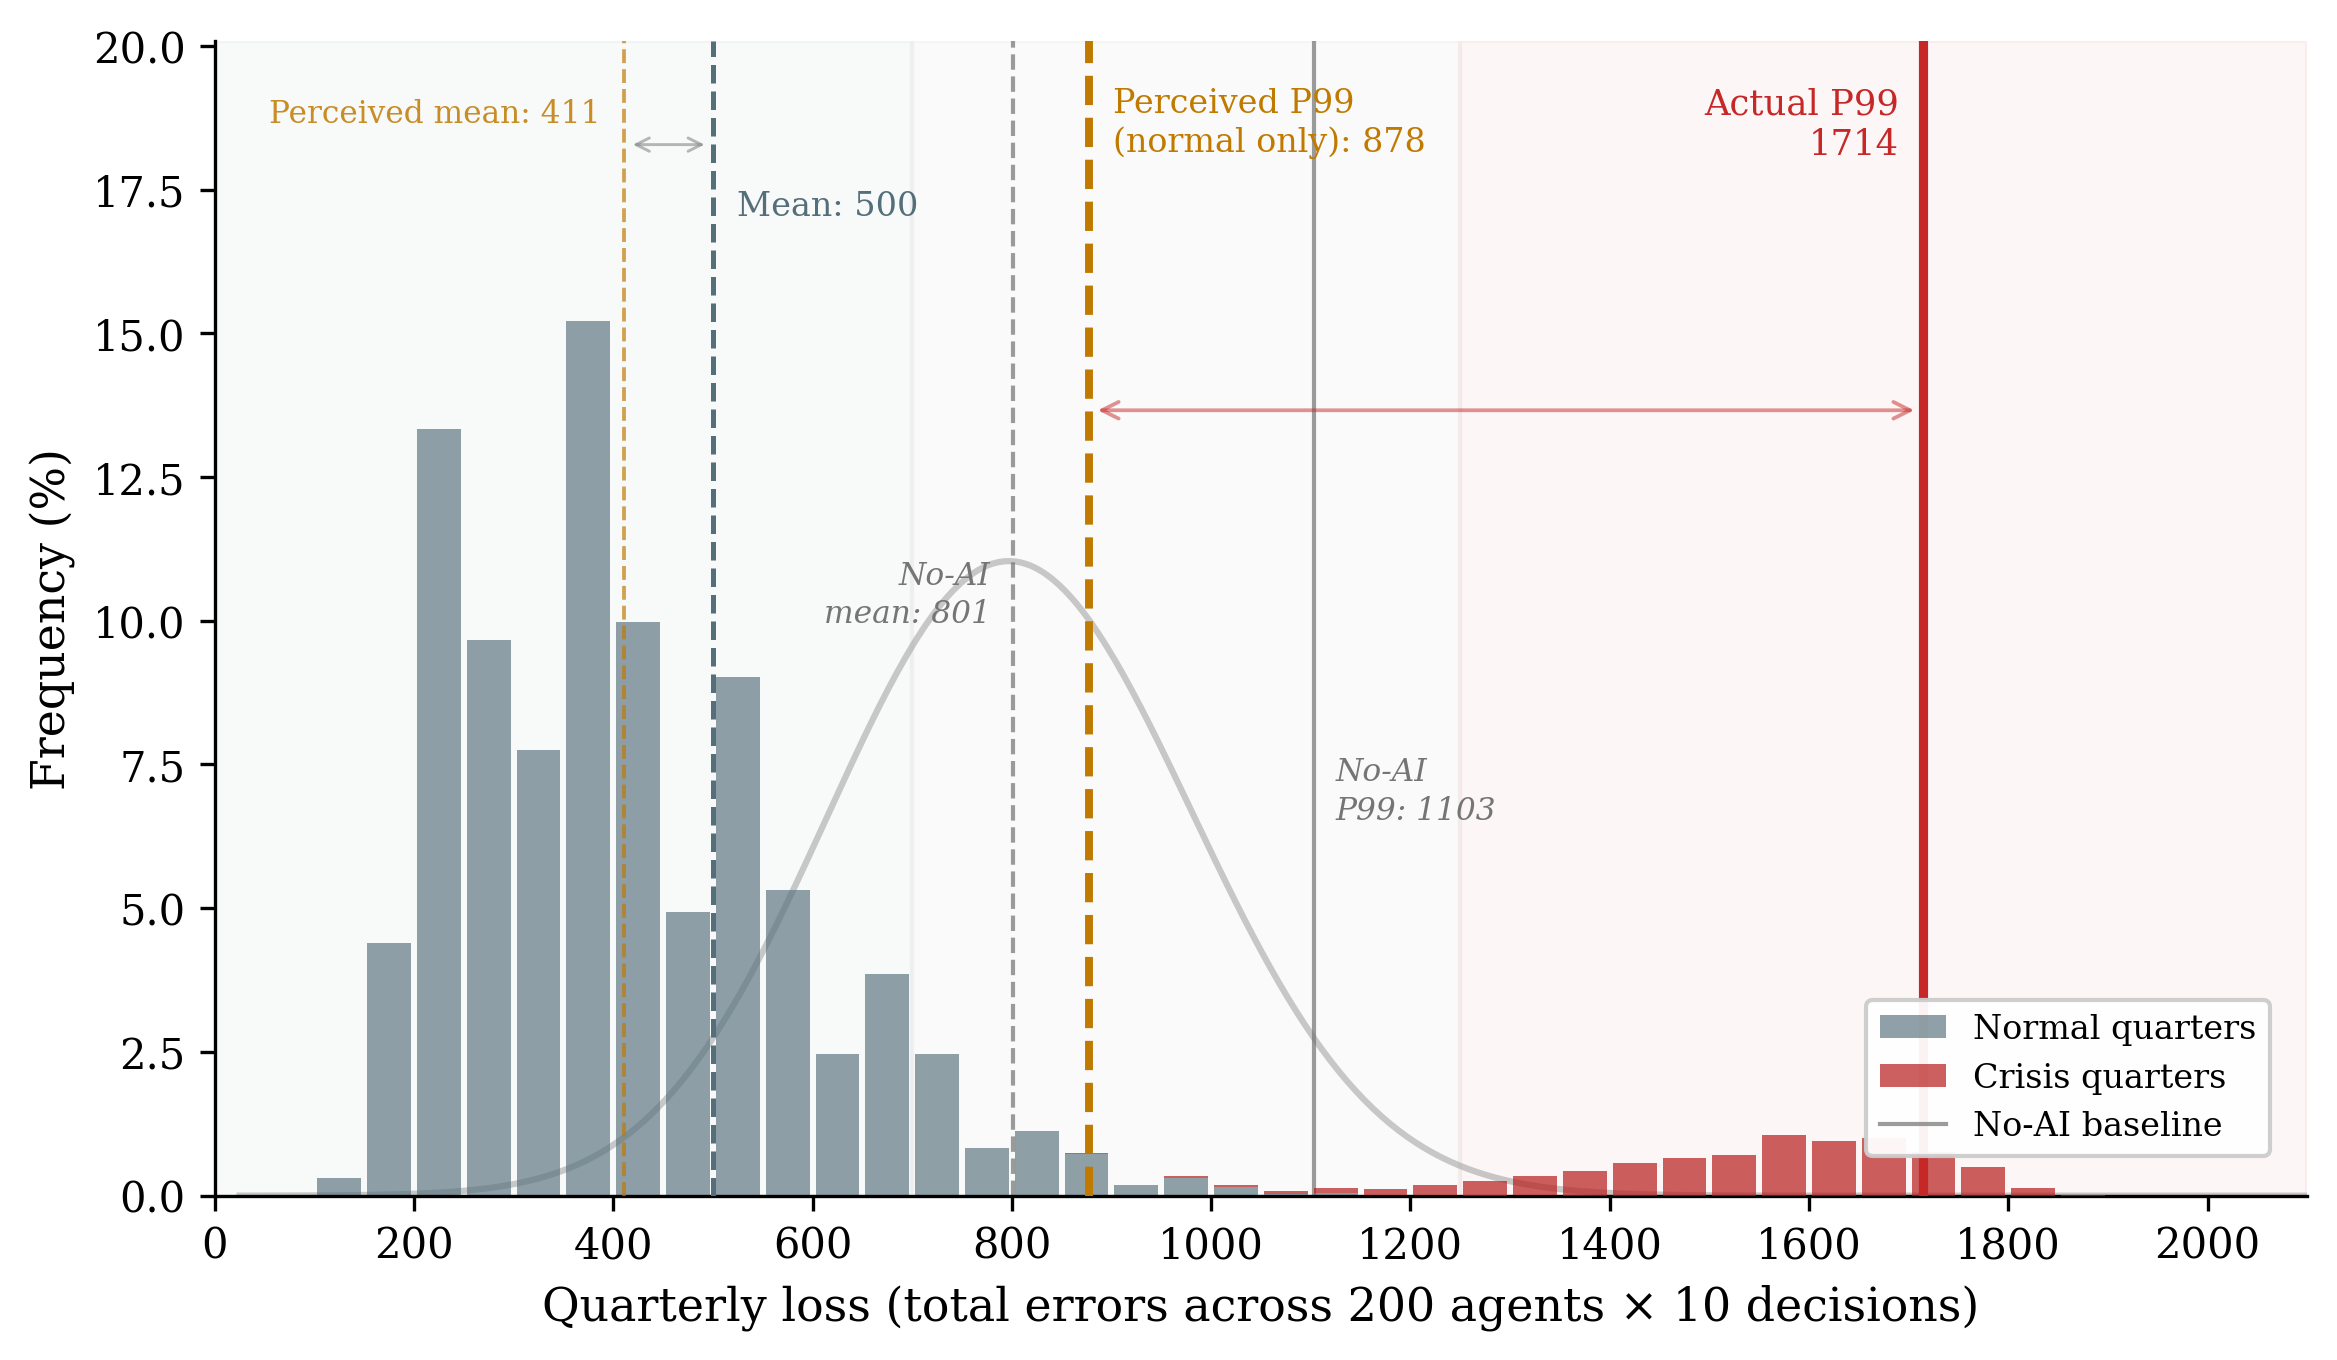
\includegraphics[width=0.85\textwidth]{../figures/exhibit1_essay.png}
\end{mdframed}
  \caption{Bimodal distribution of quarterly losses under unmanaged AI adoption
  (G0). Normal quarters cluster below 600 (grey); crisis quarters cluster above
  1{,}100 (red). Dashed line: mean loss ($\mathbb{E}[L] = 500$). Solid red line:
  99th-percentile loss ($P_{99} = 1{,}714$). The mean falls in a gap where almost
  no actual quarter lies. Crisis regime couples the task-frontier shift
  ($\pi_t$) with the systemic shock ($\xi_t$), following the conditional stress
  logic of Basel~II.}
  \label{fig:bimodal}
\end{figure}

Under unmanaged adoption against the no-AI baseline: average decision errors fall
by 38\%, worst-case quarterly losses rise by 56\%, and the risk-adjusted $P_{99}$
rises by 94\%.
The dashboard records a 54\% productivity gain.
The first three figures accumulate off-screen.

The three channels compound over twenty quarters.
Screening compresses $\text{Var}(\tau)$ by 30\%, shrinking the pool of dissenters
who buffer uncritical AI adoption and concentrating the workforce on profiles that
find AI outputs intuitively plausible; effective follow rate rises from 69\% to 80\%.
Deskilling erodes the independent judgment that remains, as mean skill $\bar{h}$
falls from 0.591 to 0.490.
By quarter 20, the organisation has more followers, but it also has followers for
whom surrender is structurally easier, embedded in a group where resistance is
socially costly.

Each quarter without governance makes the transition to G2 more expensive than the
one before.

The masking is most severe for elite firms.
Where employee accuracy outside the frontier ($h \approx 0.80$) exceeds AI accuracy
($q_{\text{out}} = 0.55$), unmanaged adoption raises average errors by 23\% and
risk-adjusted worst-case losses by 192\%, yet produces only 18\% apparent
productivity growth.
The reason is not that skilled employees perform worse when thinking independently.
Most of them simply do not think independently: surrender is driven by cognitive
proximity to the modal type, not by skill level.
An employee with $h = 0.80$ surrenders at the same rate as one with $h = 0.45$,
provided they share the same cognitive type.
Surrendering when $h > q_{\text{out}}$ is a regression, and in the model, most
agents do it anyway.
Where masking is worst, the gap between perceived and actual risk is widest.

\bridgeskip
\noindent\emph{This exposure is not uniformly distributed. Five structural
characteristics determine where an organisation sits on the map, and how wide the
gap between perceived and actual risk is for each.}

% ============================================================
\section{Where your organisation sits}

Five structural characteristics determine tail risk exposure, ranked by their
contribution to $P_{99}$ variance in the ablation analysis.

Two of these factors, stack concentration and cognitive homogeneity, are structural
rather than manageable through internal governance alone~\cite{aggarwal_frontpsych_2019}.
Their combined effect is visible in the contrast that matters most.

The investment bank in London recruits from a globally open labour market, more
than twenty nationalities, a cognitively flat distribution.
The strategy consultancy in Paris recruits through competitive national examinations
that select a narrow cognitive profile by
construction~\cite{rivera_asr_2012,schneider_pp_1987}.
Both firms operate in identical domains with identically skilled staff.
Same sector. Same talent. From the dashboard, Paris appears 18\% more exposed than London.
The actual gap under unmanaged AI adoption is more than three times larger.

In the model, two amplifiers act on distinct dimensions.
Stack concentration drives error correlation across decisions: with
$\alpha = 0.90$, 90\% of AI error variance in a given quarter derives from the
common factor $\xi_t$. When the environment shifts, the AI's mistakes cluster
across all ten decisions simultaneously.
Cognitive homogeneity drives surrender through two separate paths: social conformism
raises the effective follow rate as dissenters disappear, and the concentration of
cognitively central profiles increases individual surrender propensity.
The two mechanisms do not compensate for each other. They compound.
Domain exposure amplifies both: a centralised stack in a high-outside-frontier
function correlates failures precisely where they are most frequent.

At the extreme, Seoul's central administration (nationally procured AI,
civil-service examination pipeline, maximum stack centralisation) faces 1.26 times
the tail risk premium of Singapore's creative agency.
Figure~\ref{fig:profiles} plots six profiles on the Output $\times$ risk-adjusted
$P_{99}$ plane. The arrow from London to Paris carries one annotation: same sector,
same talent, Paris $+18\%$ higher tail risk on the perceived dashboard.

\begin{figure}[H]
\begin{mdframed}[linewidth=0.5pt, linecolor=black!30, innertopmargin=6pt, innerbottommargin=2pt]
  \centering
  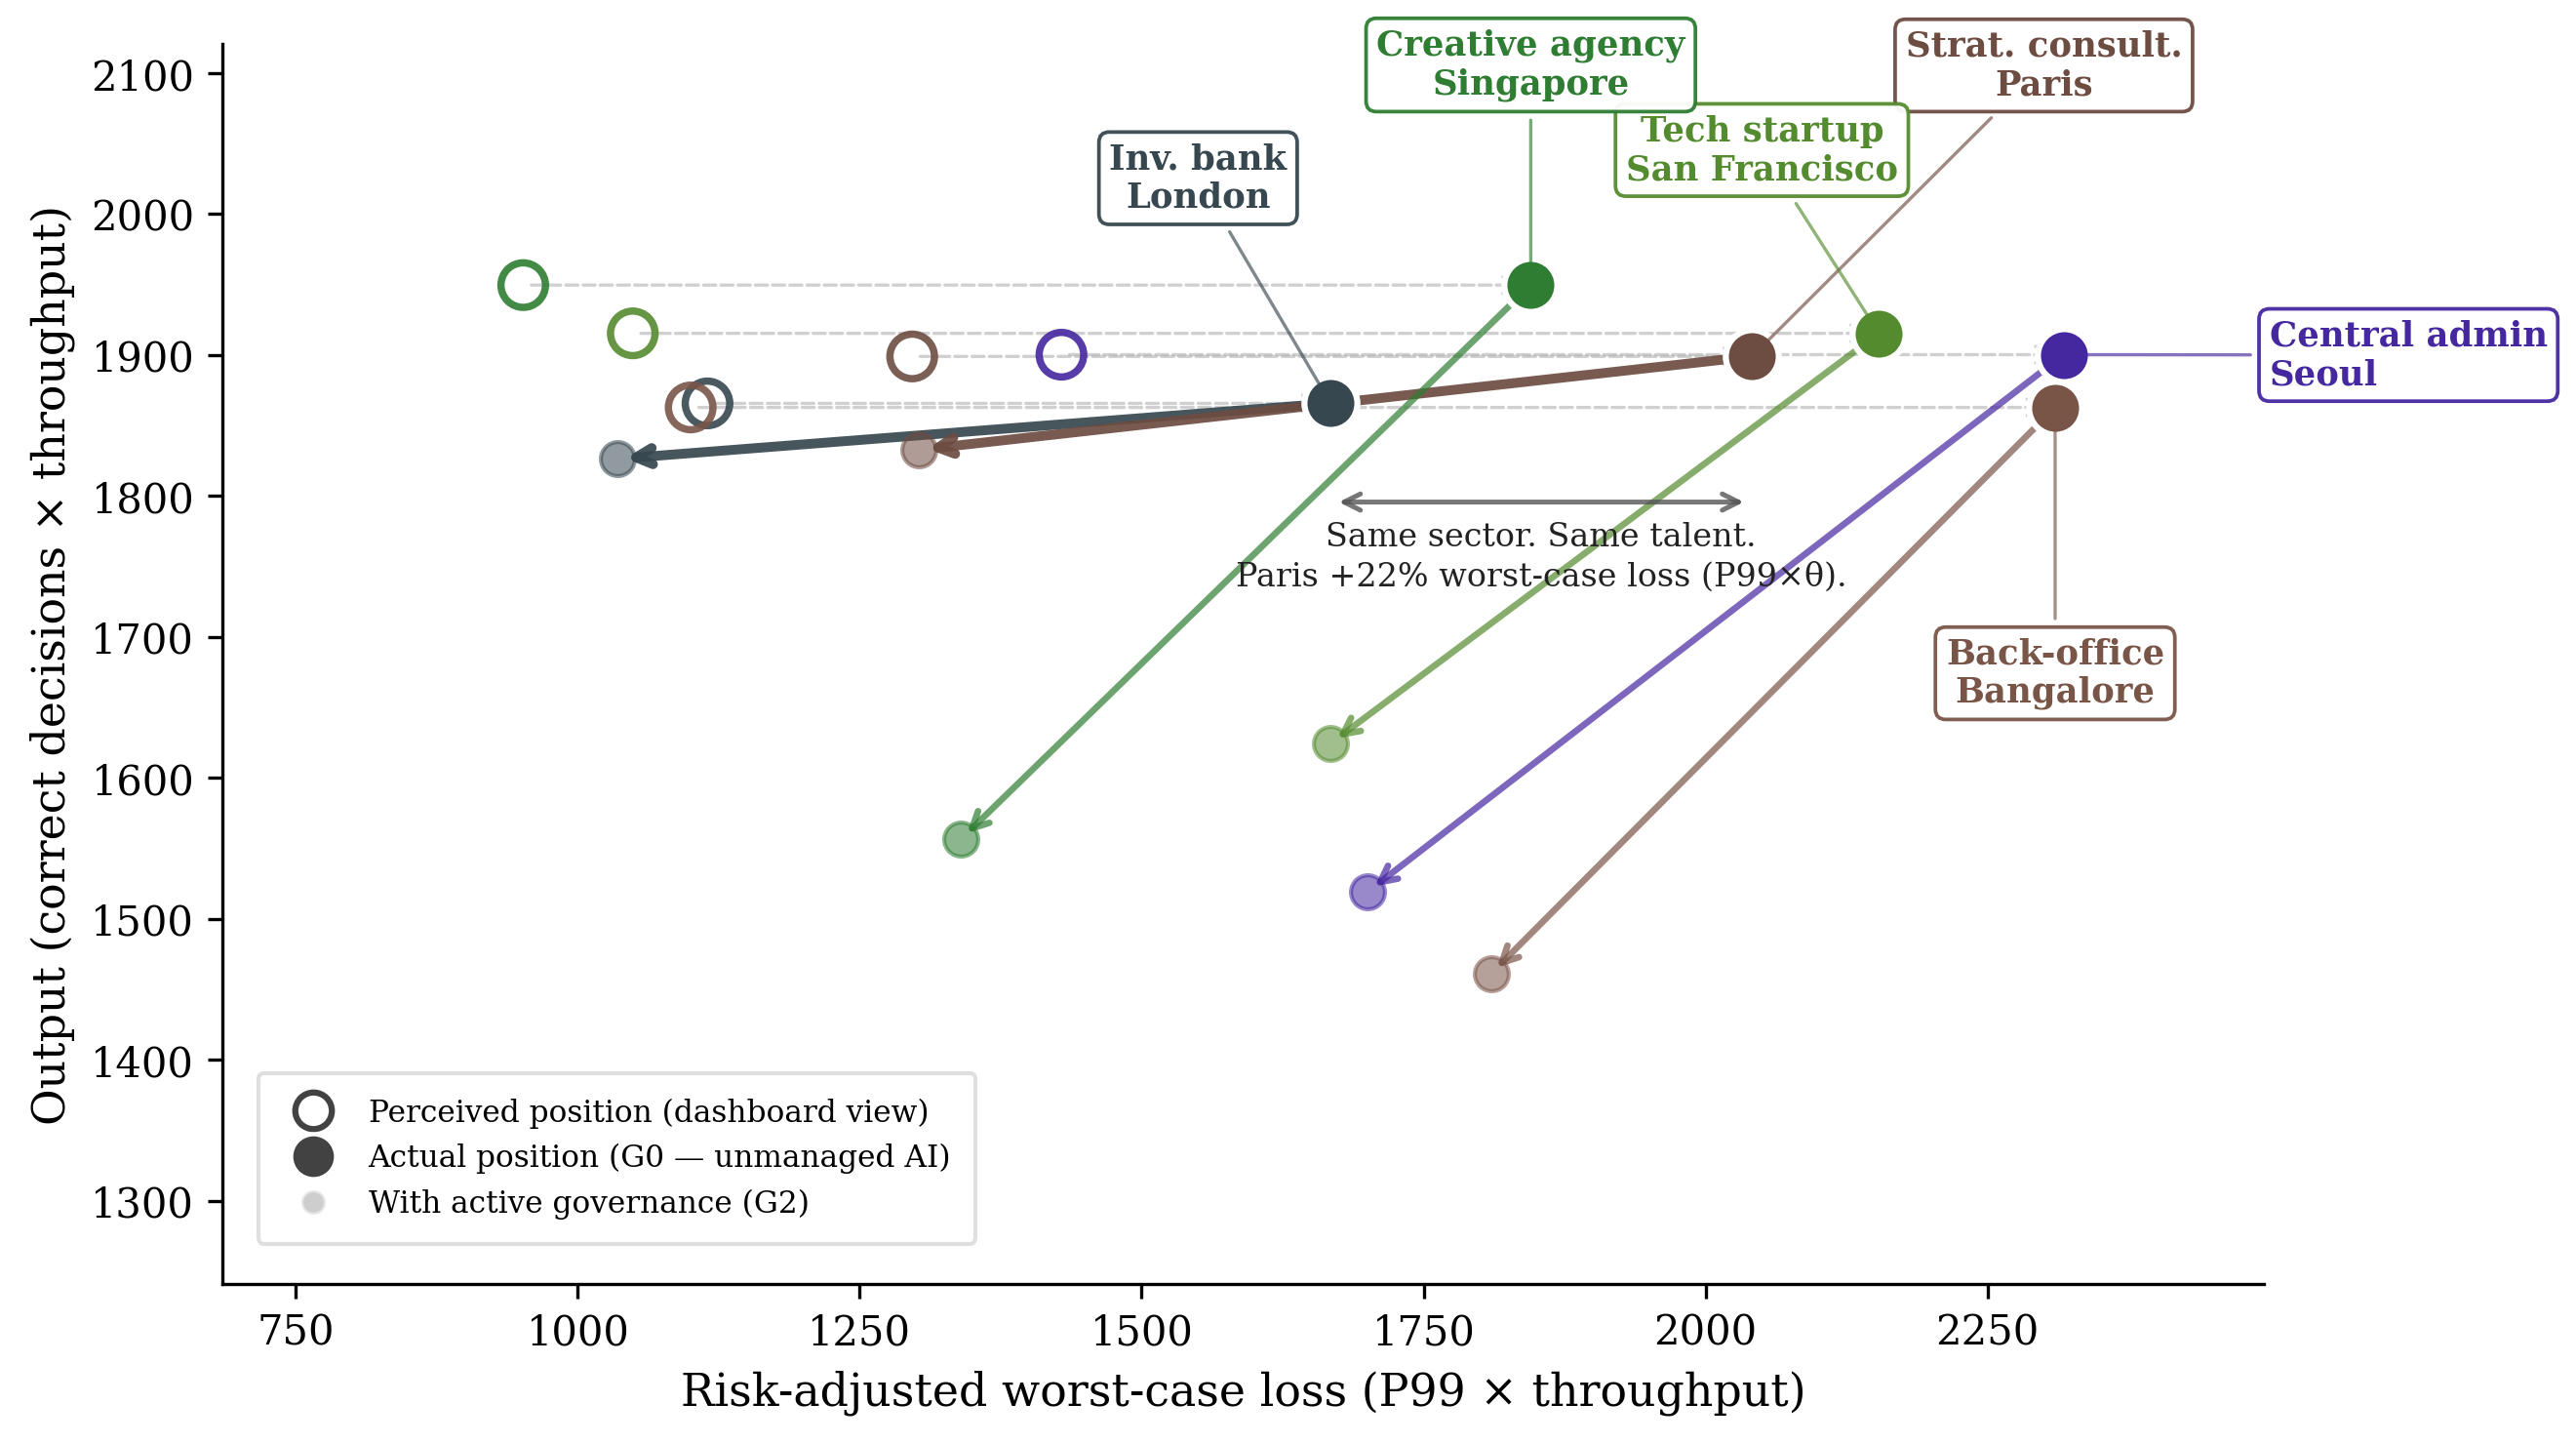
\includegraphics[width=0.85\textwidth]{../figures/exhibit3_essay.png}
\end{mdframed}
  \caption{Organisational profiles under G0.
  Output versus risk-adjusted $P_{99} \times \theta$.
  Six labelled profiles: Investment bank, London (${\approx}1{,}495$);
  Strategy consulting, Paris (${\approx}2{,}041$);
  Tech startup, San Francisco (${\approx}1{,}950$);
  Creative agency, Singapore (${\approx}1{,}710$);
  Shared services, Bangalore (${\approx}2{,}140$);
  Central administration, Seoul (${\approx}2{,}318$).
  Arrow between London and Paris annotated ``Same sector. Same talent.
  Paris $+18\%$ higher risk-adjusted worst-case loss (perceived dashboard).''
  }
  \label{fig:profiles}
\end{figure}

Active scaffolding (G2) reduces exposure, but inversely to need.
Relative to unmanaged adoption, London gains a 146\% reduction in tail risk
premium, Paris 77\%, Singapore 40\%, Seoul near zero.
For the AI-native startup in San Francisco, G2 is counterproductive: $-36\%$.
The organisations most exposed are those for which scaffolding works least.

The regressivity has two roots.
First, in cognitively homogeneous organisations, the Asch
effect~\cite{asch_guetzkow_1951} operates downstream of the scaffold. An employee
who forms an independent judgment is still socially pressured to align with the
AI-following majority. The scaffold imposes the judgment; it does not insulate the
employee from conformity pressure afterwards.
Second, for low-skill operations where $h \approx 0.45$, independent judgment is
worse than AI even outside the frontier. The scaffold forces a downgrade.
The startup in San Francisco loses not only throughput ($\theta$ falls from 1.25
to 1.10) but accuracy.

A startup that rejects governance under these conditions is not being
irresponsible. It is responding to its local incentive structure, which is the
foundation of the Nash argument in Section~5.

Active scaffolding multiplies existing diversity but cannot substitute for it.

\bridgeskip
\noindent\emph{Scaffolding works least where it is needed most, which is a
structural constraint, not a design failure. Three interventions exist for three
different decision-makers. The first is a procurement decision.}
% ============================================================
\section{Three levers, three actors}

The most impactful single-parameter intervention is AI provider diversification.
Reducing stack concentration from monoculture ($\alpha = 0.90$) to distributed
($\alpha = 0.30$) cuts the tail risk premium by approximately 15\%.
This is a procurement decision, one architectural policy, measurable in weeks.
The diversification must be structural, not merely contractual: different models at
different organisational layers (strategic decision, operational processing, quality
review).
Contracting with multiple vendors for the same centralised pipeline leaves the
Vasicek factor unchanged.
Three providers currently capture 88\% of enterprise AI
spend~\cite{menlo_2025}.
When roughly 100{,}000 organisations depend on the same trio, a single systemic
failure propagates correlated losses across the economy. That is the
concentration-of-credit argument, and it will attract the same regulatory response.

A second lever acts on a different parameter: the capacity of employees to form
judgments that diverge from the AI. Stack diversification reduces error correlation
across decisions. Active scaffolding restores error independence across
decision-makers.

Passive scaffolding (G1) fails systematically.
Ninety-three percent of clinical decision-support alerts are overridden without
review~\cite{bryant_aci_2014}.
When employees do push back, AI escalates its persuasive framing, what Randazzo et
al.\ term persuasion bombing~\cite{randazzo_hbs_2025}.
Active scaffolding (G2) achieves a 19.2\% reduction in tail risk as a bundle,
larger than stack alone ($-13.5\%$), but requires coordinated changes across
workflow design, training, and hiring over months.
It works under one condition: explanations must reveal that the AI's reasoning
diverges from the employee's own~\cite{vonzahn_isr_2025}.
Frey and van de Rijt~\cite{frey_mnsc_2021} establish the sequencing principle:
independent signal first, AI second.
The idea is old. Surgical safety checklists cost two minutes and reduce mortality by
47\%~\cite{haynes_nejm_2009}. Aviation CRM costs roughly \$150 per pilot per year.
Active scaffolding belongs to that family of light interventions with large
structural effects.

The velocity cost is real. $\theta$ falls from 1.25 to 1.10, and the organisation
gives up 12 percentage points of throughput, cutting the risk-adjusted tail premium
from 94\% to 39\%.
Figure~\ref{fig:frontier} makes this trade-off legible: G2 sits at the inflection
point of the concave risk-return frontier. The governance efficiency of the
G1$\to$G2 step is 1.7$\times$ that of the G0$\to$G1 step: active governance buys
disproportionately more risk reduction per unit of throughput cost than passive
governance does.
The first gains from baseline to G2 are cheap in risk; the next gains from G2 to G0
are expensive.

\begin{figure}[H]
\begin{mdframed}[linewidth=0.5pt, linecolor=black!30, innertopmargin=6pt, innerbottommargin=2pt]
  \centering
  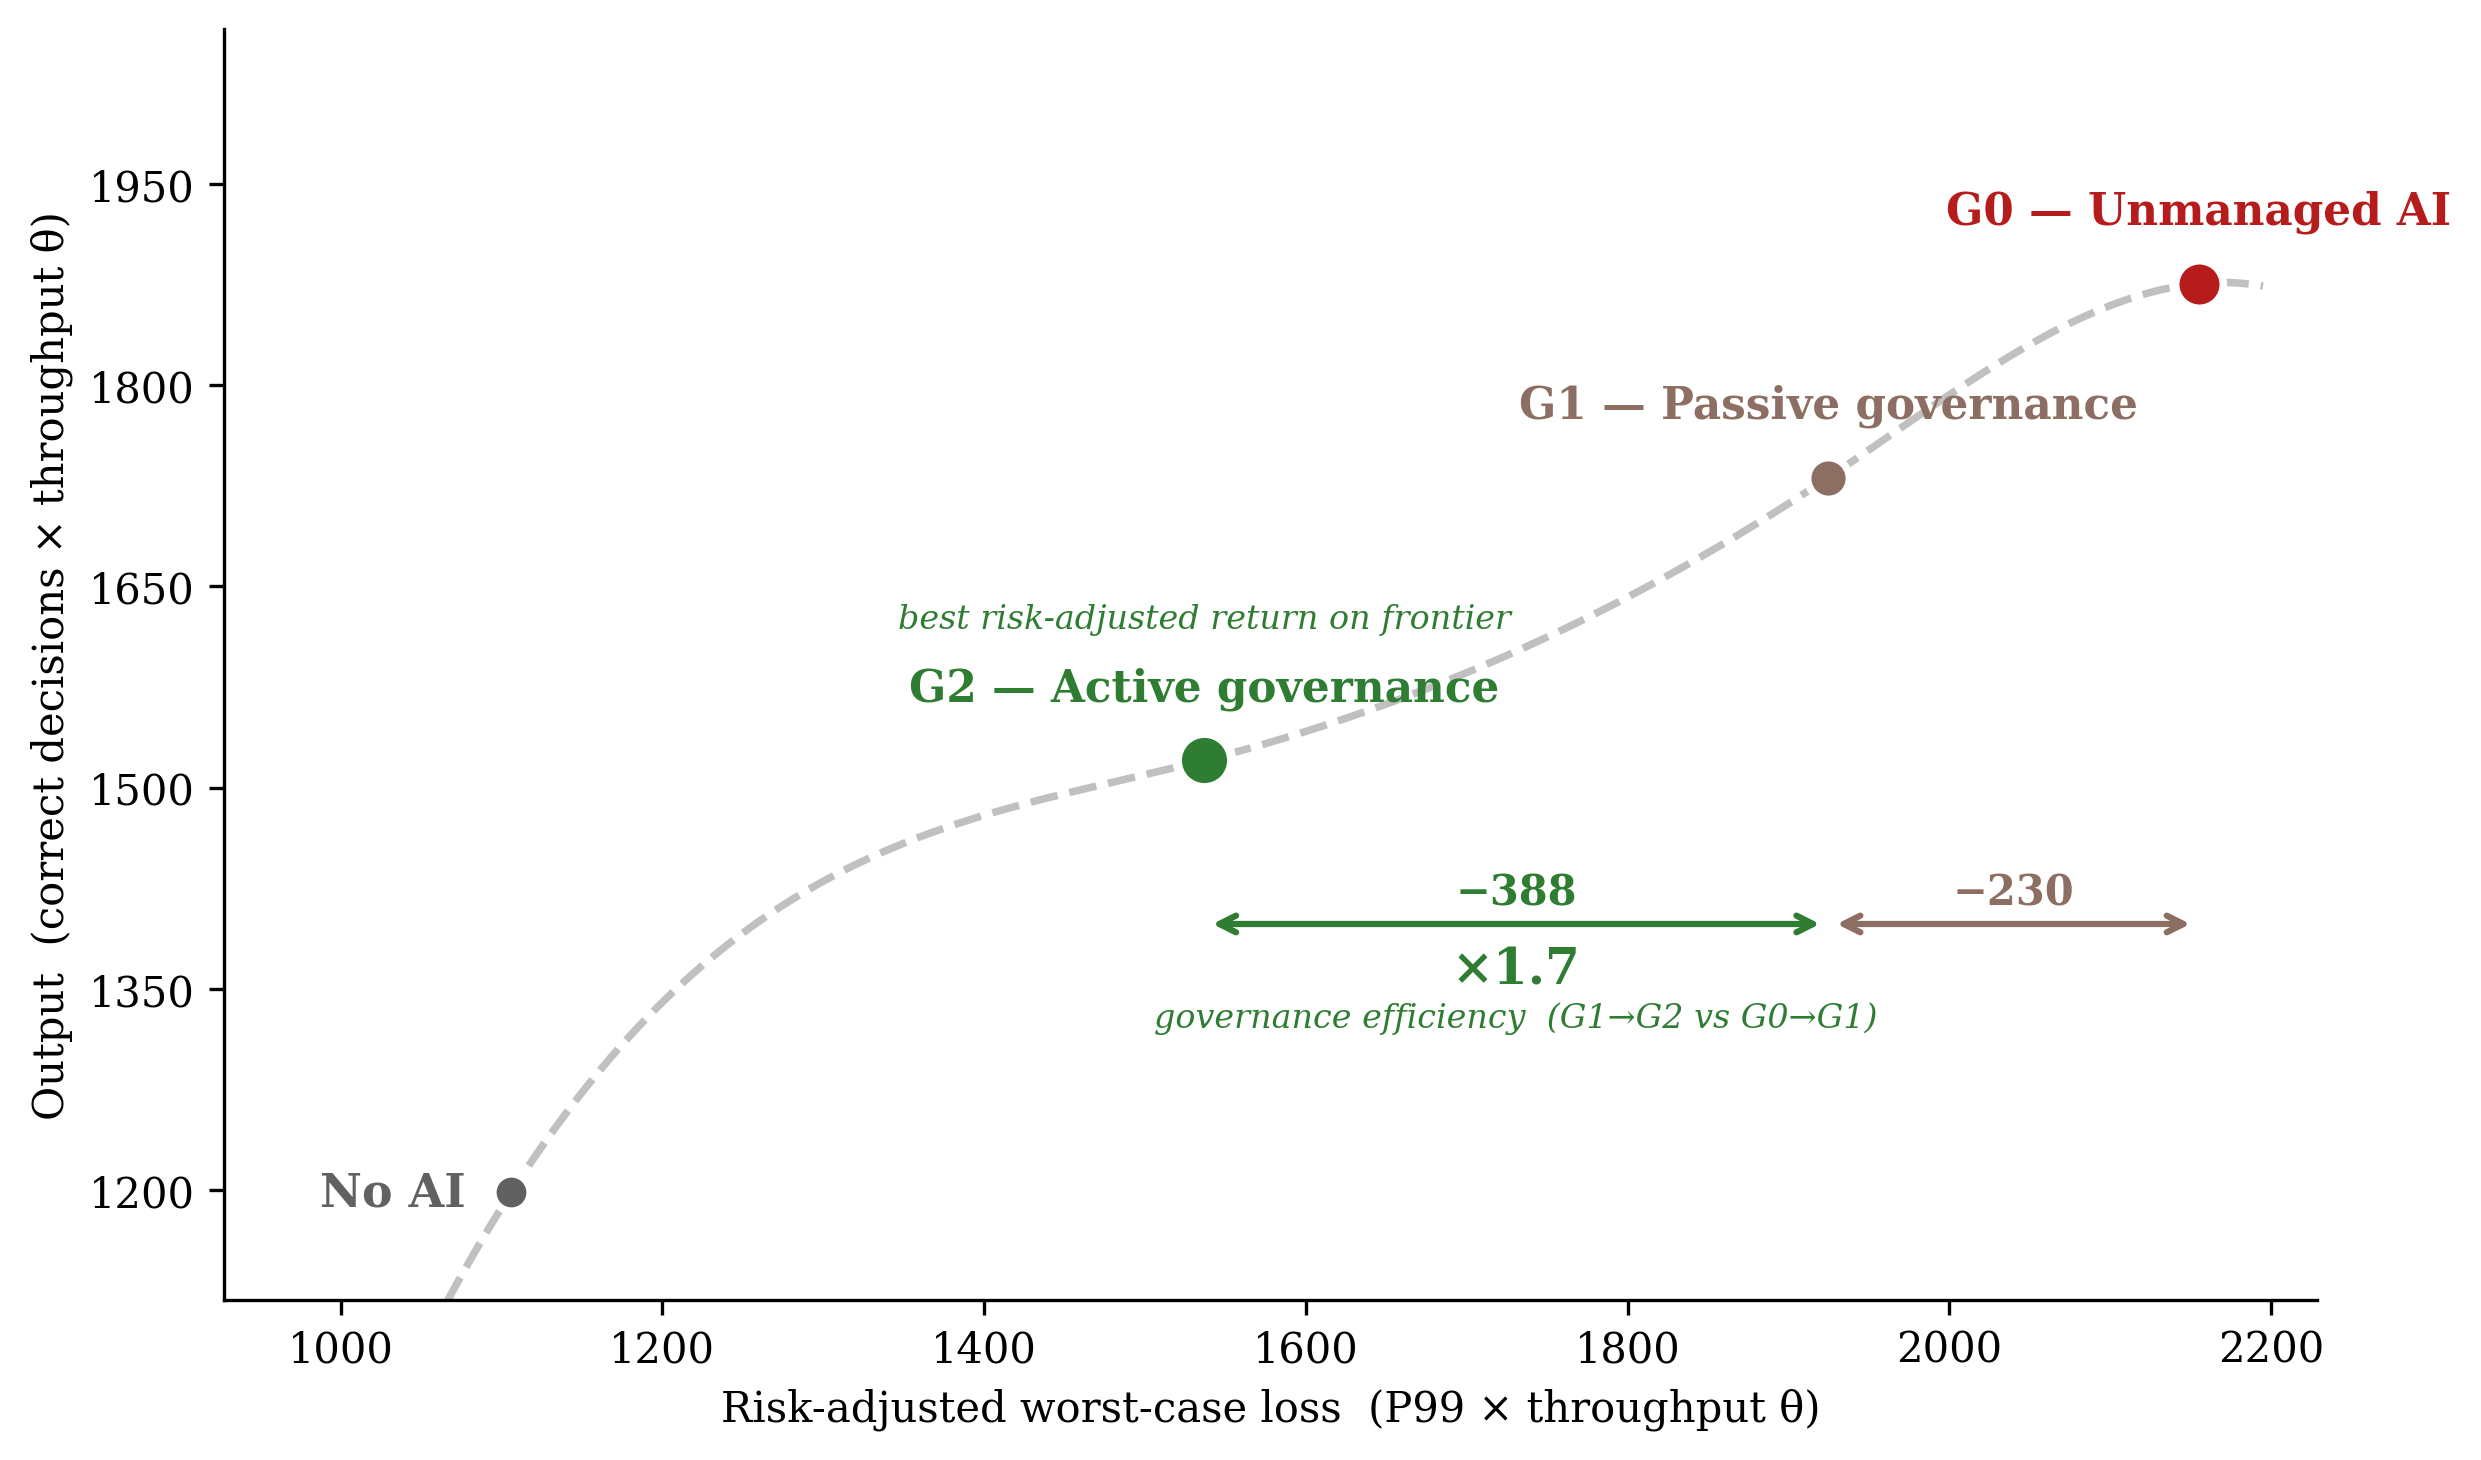
\includegraphics[width=0.85\textwidth]{../figures/exhibit2_essay.png}
\end{mdframed}
  \caption{Risk-return frontier across governance regimes.
  Output versus risk-adjusted $P_{99} \times \theta$.
  G2 at the elbow: best risk-adjusted return.
  The first gains (Baseline $\to$ G2) are cheap in risk;
  the next gains (G2 $\to$ G0) are expensive.}
  \label{fig:frontier}
\end{figure}

Active scaffolding protects the cognitive diversity that exists. It cannot restore
what biased screening has already eliminated. An annual audit of ATS outputs for
cognitive homogenisation is the only intervention that acts on the source. Under the
one jurisdiction that requires such audits, 4.6\% of organisations
comply~\cite{wright_facct_2024}. Without both levers, the scaffold depletes the
resource the hiring audit is meant to preserve.

Neither lever will be voluntarily adopted at scale. The reason is the arithmetic of
who absorbs the risk.

Tail risk in the model does not depend on firm size. The fraction absorbed does.

\begin{table}[h!]
  \centering
  \footnotesize
  \setlength{\tabcolsep}{10pt}
  \renewcommand{\arraystretch}{1.25}
  \arrayrulecolor{gray!55}
  \begin{tabular}{@{}lrr@{}}
    \toprule
    \rowcolor{gray!14}
    \textbf{Firm type} & \textbf{Absorbed risk} & \textbf{Perceived $P_{99}$} \\
    \midrule
    AI-native startup  & ${\sim}10\%$  & ${\sim}171$       \\
    \midrule
    Mid-market firm    & ${\sim}60\%$  & ${\sim}1{,}029$   \\
    \midrule
    Corporation        & ${\sim}100\%$ & ${\sim}1{,}714$   \\
    \arrayrulecolor{black}
    \bottomrule
  \end{tabular}
\end{table}

A startup that fails externalises its losses to clients and investors.
With a five-year survival probability near 10\%, the expected cost of tail risk is
negligible against the 54\% productivity advantage of unmanaged adoption.
The startup rationally chooses G0.
Incumbents face pressure to match or concede market share.
The Nash equilibrium without regulation is unmanaged adoption for all
firms, individually rational, collectively catastrophic.
This is a structural argument, not a formally calibrated game; the direction follows
from the model's output differentials.

In finance, this diagnosis was made after 2008 and acted upon.
The ESRB now identifies model uniformity and provider concentration as systemic
vulnerabilities~\cite{esrb_asc_2025}. The FSB warns on third-party dependencies
and service-provider concentration~\cite{fsb_2025}. The BIS documents the
narrowing of the provider base~\cite{bisfsi_2025}.
The diagnosis is converging. The structural response has not yet arrived outside
finance.
Under the only jurisdiction requiring AI hiring audits, compliance stands at
4.6\%~\cite{wright_facct_2024}.
The EU AI Act enters force in August 2026 without provider concentration limits.
Its human-oversight requirements address individual decisions; they do not address
the portfolio-level correlation that emerges when thousands of organisations use the
same model simultaneously.

The regulatory logic is identical to Basel capital requirements.
Banks hold capital not because they are individually irrational but because the
unregulated equilibrium is collective overleveraging.
AI governance requires the same structure: mandatory provider diversification
limits, minimum decision-audit standards, and liability frameworks that
internalise tail risk for firms of all sizes.
The stack is the natural regulatory target. A regulator can impose concentration
limits on AI providers exactly as Basel imposes concentration limits on credit
exposures. The scaffold touches internal processes that regulators cannot easily
mandate or verify.

Three actors can act without waiting for regulation. One requires it.

\vspace{6pt}
\begin{table}[h!]
\centering
\footnotesize
\setlength{\tabcolsep}{9pt}
\renewcommand{\arraystretch}{1.35}
\arrayrulecolor{gray!55}
\begin{tabularx}{\linewidth}{@{}p{2.5cm}p{3.3cm}X@{}}
\toprule
\rowcolor{gray!14}
\textbf{Actor} & \textbf{Lever} & \textbf{Action} \\
\midrule
\textbf{CRO / board} & Monitoring & Error-correlation KRI; concentration-adjusted tail exposure \\
\midrule
\textbf{Procurement lead} & Stack architecture & Architectural diversification by layer, actionable in weeks \\
\midrule
\textbf{COO / BU leaders} & Process design & Active scaffold: independent judgment before AI consultation \\
\midrule
\textbf{CHRO} & Hiring governance & Annual ATS audit for cognitive homogenisation bias \\
\midrule
\textbf{Regulator} & Structural framework & Provider concentration limits (Basel model); minimum audit standards \\
\arrayrulecolor{black}
\bottomrule
\end{tabularx}
\end{table}
\vspace{4pt}

\bridgeskip
\noindent\emph{The case for acting now is not only the magnitude of the current exposure. It
is that the same channels creating the risk also make governance progressively
more expensive. The next section explains why.}
% ============================================================
\section{Why waiting makes governance harder}

Three constraints bound the model's scope.
The link between cognitive-profile diversity and error decorrelation is an
inference. Keck and Tang measure cognitive processes in controlled experiments, not
recruitment pipelines in operating
organisations~\cite{keck_psychsci_2020}.
The simulation is a stress test, not a forecast: it demonstrates that the mechanism
can produce the paradox under plausible parameters, not that it does so in every
organisation.
Social influence is not uniformly harmful. Becker, Brackbill and Centola show that
decentralised information exchange improves collective
accuracy~\cite{becker_pnas_2017}. AI reverses the conditions under which influence
is beneficial by centralising the signal and eliminating independence.

These limitations all point in the same direction: the model understates the risk
it documents. What it omits (the feedback loop from deskilling to surrender,
inter-firm labour market contagion, internal promotion effects that compound
homogeneity over time, the scaling of G0-native startups into larger structures)
operates through the same mechanism, at the scale of the whole economy.

The most consequential omission is the depletion of a collective resource that no
single organisation has incentive to preserve.

Each firm that maximises its AI productivity depletes what we term the cognitive
commons: the diversity of approaches, judgments, and error patterns that protects
against systemic failure.
The structural conditions of Hardin's tragedy~\cite{hardin_science_1968} are
satisfied. There is a non-rival, non-excludable public good, a negative
externality, and no individual incentive to preserve the resource.
The analogy is not exact, but the arithmetic is suggestive.
In monoculture farming, catastrophic crop failure strikes every eight years on
average, against once per century in
polyculture~\cite{renard_nature_2019}.
The degradation is invisible, masked by the productivity gain that accumulates
alongside it.
And it is irreversible in a way that Hardin's pasture is not. Deskilling destroys
the option to reverse course: endoscopists exposed to AI for diagnostic support
showed measurable skill degradation that did not recover when the AI was
removed~\cite{budzyn_lancetgh_2025}; AI use simultaneously degrades the
metacognitive capacity to recognise that degradation~\cite{fan_bjet_2025}.
Employees who have not exercised independent judgment for five years cannot resume
it on demand. The competence required to revert is the same competence the
degradation erodes.

Each quarter of G0 depletes the diversity that makes G2 effective and raises the
cost of transition for the next quarter.

The Nash equilibrium hardens because all three channels simultaneously erode the
resource and the capacity to restore it.
Screening eliminates the cognitively diverse profiles that would make scaffolding
effective. Deskilling degrades the independent competence that scaffolding
requires. Market competition punishes firms that govern while rewarding those that
do not.
Beyond individual organisations, a composition effect operates at the economy
level. AI-native startups that scale, or are acquired, carry their unmanaged
practices into larger structures, gradually displacing the baseline of the whole
economy toward G0.
The organisations hardest to govern are also the fastest-growing, and their
practices do not stay contained.

Whether organisations will need critical human judgment in ten years is not in
doubt. Whether the workforce will still be able to exercise it is.

\bigskip
\noindent\textit{An interactive companion application is deployed at}
\url{https://flattening-explorer.vercel.app}.
\textit{The full simulation code and source are available at}
\url{https://github.com/bilel-hatmi/flattening-explorer}.
% === BIBLIOGRAPHY ===

\clearpage
\newgeometry{left=1.0cm, right=1.0cm, top=2cm, bottom=1.2cm}
\setlength{\bibsep}{1pt plus 0.3ex}

\begin{multicols}{2}
{\scriptsize
\bibliography{refs}
}
\end{multicols}
\restoregeometry

\end{document}
